\begin{figure}[htbp]
\section*{ SETD2}
\centering
\begin{subfigure}[b]{0.65\textwidth}
\centering
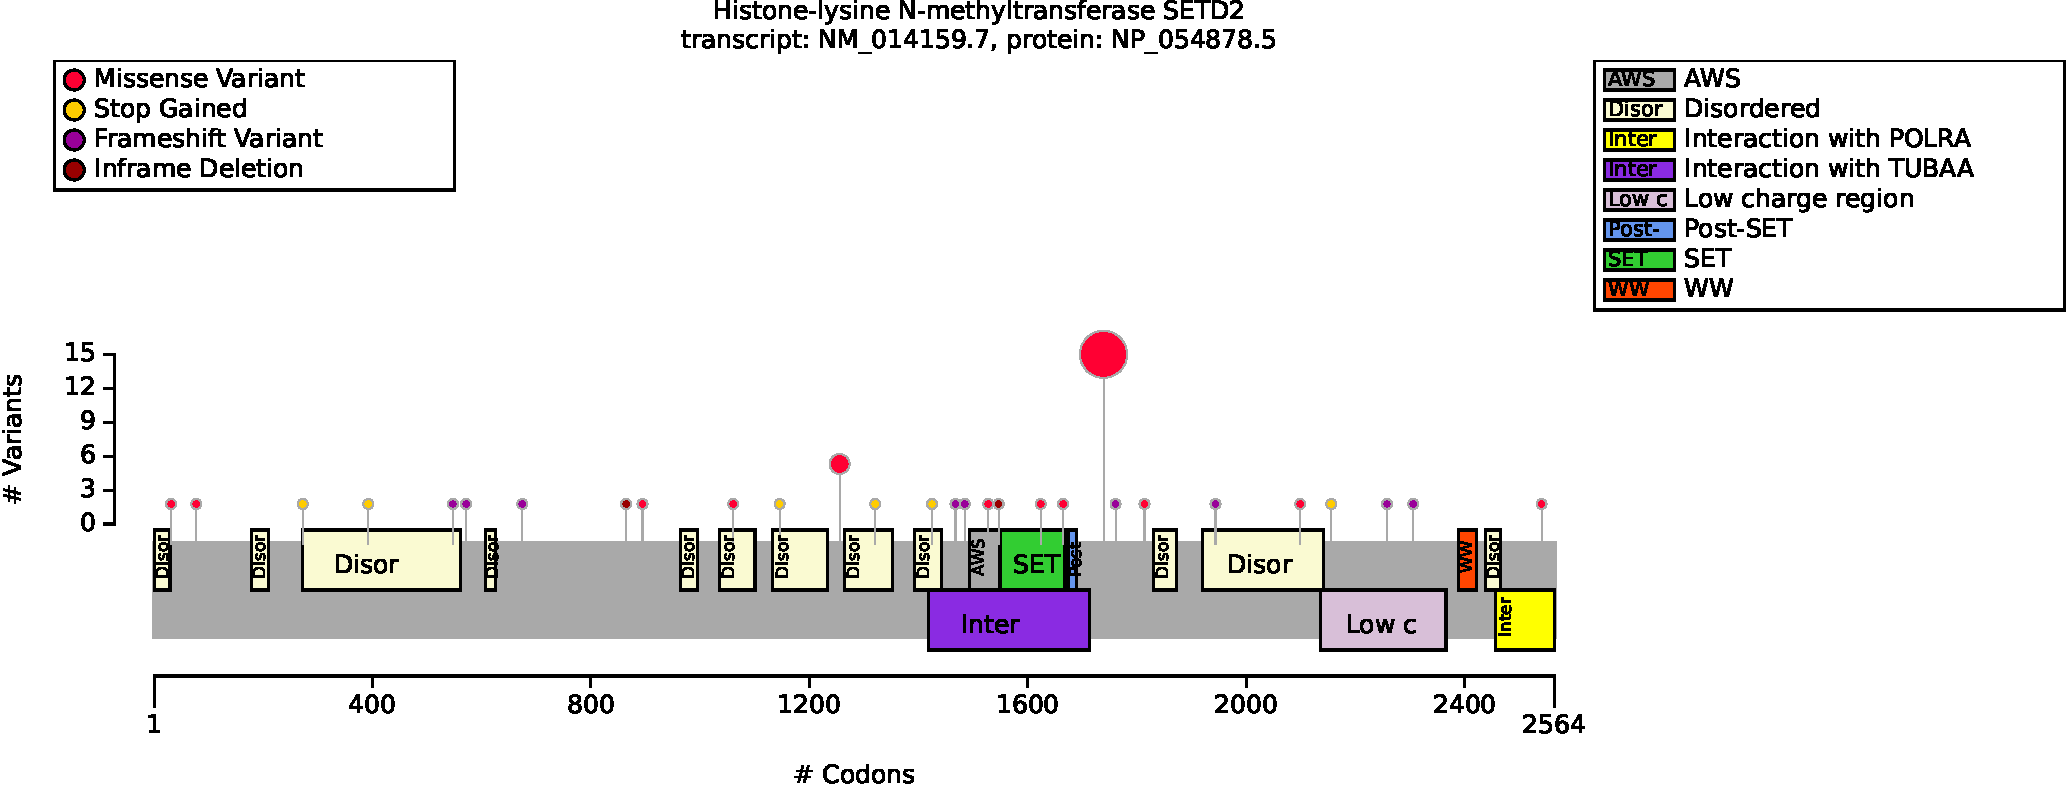
\includegraphics[width=\textwidth]{img/SETD2_protein_diagram.pdf} 
\captionsetup{justification=raggedright,singlelinecheck=false}
\caption{Distribution of variants in SETD2}
\end{subfigure}
\begin{subfigure}[b]{0.3\textwidth}
\centering
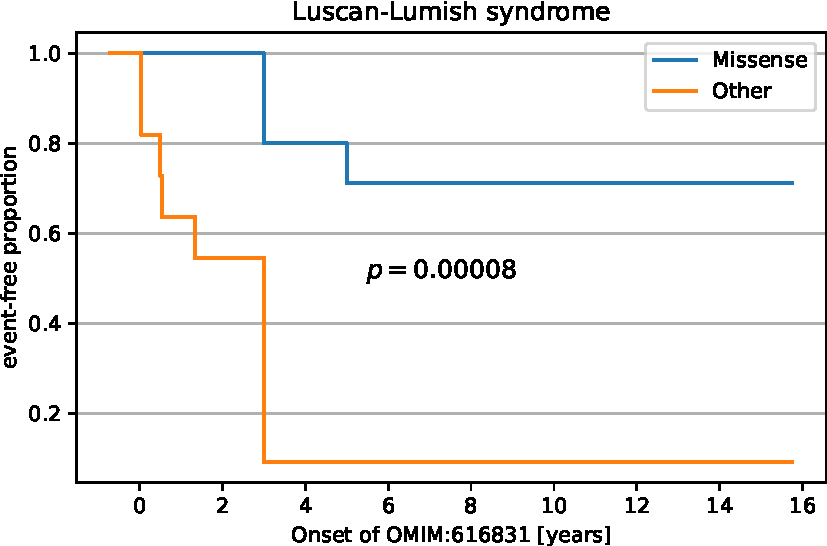
\includegraphics[width=1\textwidth]{ img/SETD2_stats.pdf} 
\captionsetup{justification=raggedright,singlelinecheck=false}
\caption{Luscan-Lumish syndrome onset. }
\end{subfigure}

\vspace{0.5em}

\begin{subfigure}[b]{\textwidth}
\centering
\resizebox{\textwidth}{!}{
\begin{tabular}{llllrr}
\toprule
HPO term & Arg1740Trp & Other & p-value & adj. p-value\\
\midrule
Severe global developmental delay [HP:0011344] & 9/9 (100\%) & 0/12 (0\%) & $3.40\times 10^{-6}$ & $8.17\times 10^{-5}$\\
Hypertelorism [HP:0000316] & 11/11 (100\%) & 5/23 (22\%) & $1.53\times 10^{-5}$ & $1.83\times 10^{-4}$\\
Macrocephaly [HP:0000256] & 0/11 (0\%) & 19/28 (68\%) & $1.45\times 10^{-4}$ & 0.001\\
Delayed ability to walk [HP:0031936] & 8/8 (100\%) & 1/10 (10\%) & $4.11\times 10^{-4}$ & 0.002\\
Scoliosis [HP:0002650] & 6/6 (100\%) & 2/14 (14\%) & $7.22\times 10^{-4}$ & 0.003\\
Wide nasal bridge [HP:0000431] & 9/9 (100\%) & 2/9 (22\%) & 0.002 & 0.009\\
Ventriculomegaly [HP:0002119] & 4/4 (100\%) & 2/17 (12\%) & 0.003 & 0.009\\
\bottomrule
\end{tabular}
}
\captionsetup{justification=raggedright,singlelinecheck=false}
\caption{Fisher Exact Test:HPO annotation frequency vs. Arg1740Trp / Other. Total of
        24 tests were performed.}
\end{subfigure}
\vspace{0.5em}
\begin{subfigure}[b]{0.95\textwidth}
\centering
\resizebox{\textwidth}{!}{
\begin{tabular}{llllrr}
\toprule
HPO term & Missense & Other & p-value & adj. p-value\\
\midrule
Macrocephaly [HP:0000256] & 4/24 (17\%) & 15/15 (100\%) & $1.54\times 10^{-7}$ & $4.16\times 10^{-6}$\\
\bottomrule
\end{tabular}
}
\captionsetup{justification=raggedright,singlelinecheck=false}
\caption{Fisher Exact Test: HPO annotation frequency vs. Missense / Other. Total of 27 tests were performed.}
\end{subfigure}
\vspace{0.5em}
\begin{subfigure}[b]{0.95\textwidth}
\centering
\resizebox{\textwidth}{!}{
\begin{tabular}{llllrr}
\toprule
Genotype (A) & Genotype (B) & total tests performed & significant results\\
\midrule
FEMALE & MALE & 27 & 0\\
\bottomrule
\end{tabular}
}
\captionsetup{justification=raggedright,singlelinecheck=false}
\caption{Fisher Exact Test performed to compare HPO annotation frequency with respect to genotypes.}
\end{subfigure}

\begin{subfigure}[b]{0.95\textwidth}
\captionsetup{justification=raggedright,singlelinecheck=false}
\resizebox{\textwidth}{!}{
\begin{tabular}{llllrr}
\toprule
Description & Variable & Genotype (A) & Genotype (B) & p-value & xrefs\\
\midrule
Luscan-Lumish syndrome (OMIM:616831) onset & Onset of OMIM:616831 & Missense & Other & $8.47\times 10^{-5}$ & -\\
\bottomrule
\end{tabular}
}
\caption{Onset of OMIM:616831 to compare Missense and Other variant. }
\end{subfigure}

\caption{The cohort comprised 45 individuals (18 females, 27 males). 1 of these individuals was reported to be deceased. 
A total of 202 HPO terms were used to annotate the cohort. 
Disease diagnoses: Luscan-Lumish syndrome (OMIM:616831) (28 individuals), 
Rabin-Pappas syndrome (OMIM:620155) (14 individuals), 
Intellectual developmental disorder, autosomal dominant 70 (OMIM:620157) (3 individuals). 
Van Nieuwenhove et al. (2020) stated that 
the origin of clinical diversity in patients with SEC61A1 mutation is currently unclear \cite{PMID_32325141}. 
Rabin et al. (2023) found that variants in codon 1740 of SETD2 whose features differ from those with LLS \cite{PMID_32710489}.
A total of 45 unique variant alleles were found in \textit{SETD2} (transcript: \texttt{NM\_014159.7}, protein id: \texttt{NP\_054878.5}).}
\end{figure}
